\section{Results}
\label{sec:results}

\begin{figure}[t]
\centering
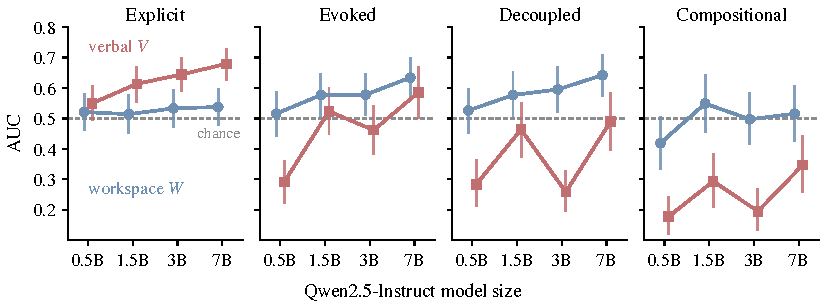
\includegraphics[width=\textwidth]{figures/fig2_regime_map.pdf}
\caption{AUC of the workspace readout ($\Wrr$), the verbal report ($\Vrep$), and
embedding relevance across model sizes (Qwen2.5-Instruct) and provenance regimes;
error bars are 95\% item-bootstrap CIs, the gray line marks chance. The two
channels trade places as provenance shifts from explicit to inferred; on the
construct-valid Decoupled benchmark the verbal report stays at or below chance at every
size. \updated{This original regime-map visualization is retained; corrected
v3 numerical results appear in the accompanying tables.}}
\label{fig:regime}
\end{figure}

\begin{table}[tbp]
\centering
\caption{Workspace and verbal ranking by provenance regime for the checkpoints discussed in the main text. Each entry is the pooled item-level AUC of the workspace readout $W$ or the verbal report $V$ (log-space yes-versus-no score through the chat template) for recovering load-bearing candidates. The first block holds three capable-scale instruct checkpoints from other families; the second is the dense Qwen3 ladder, whose 8B row is the fourth cross-family model. All 23 checkpoints appear in Table~\ref{tab:appA1}.}
\label{tab:master}
\footnotesize
\setlength{\tabcolsep}{3.8pt}
\begin{tabular}{l*{8}{c}}
\toprule
 & \multicolumn{2}{c}{Explicit} & \multicolumn{2}{c}{Evoked} & \multicolumn{2}{c}{Decoupled} & \multicolumn{2}{c}{Compositional} \\
\cmidrule(lr){2-3}\cmidrule(lr){4-5}\cmidrule(lr){6-7}\cmidrule(lr){8-9}
Model & $W$ & $V$ & $W$ & $V$ & $W$ & $V$ & $W$ & $V$ \\
\midrule
Qwen2.5-7B-Instruct & .5376 & .6792 & .6341 & .5856 & .6423 & .4897 & .5156 & .3472 \\
OLMo-2-7B-Instruct & .4938 & .6231 & .6688 & .5398 & .6664 & .3529 & .5341 & .2944 \\
Mistral-7B-Instruct-v0.3 & .5324 & .6191 & .6687 & .5777 & .6713 & .4700 & .5962 & .3242 \\
\midrule
Qwen3-1.7B & .4818 & .5917 & .5409 & .3895 & .5607 & .1961 & .4162 & .1812 \\
Qwen3-4B & .5090 & .6496 & .5744 & .4798 & .5291 & .3967 & .5050 & .2600 \\
Qwen3-8B & .5090 & .7100 & .6204 & .4534 & .6545 & .3872 & .5466 & .2079 \\
Qwen3-14B & .5083 & .7400 & .6390 & .5219 & .6677 & .4271 & .5086 & .2163 \\
Qwen3-32B & .5084 & .7480 & .6139 & .5511 & .6919 & .4782 & .5532 & .2774 \\
\bottomrule
\end{tabular}
\end{table}


\subsection{A Provenance-Dependent Dissociation}
\label{sec:dissociation}

\updatedparagraph{Table~\ref{tab:master} gives the corrected v3 grid. Across
the four capable-scale families, Decoupled $W{-}V$ is $+0.1526$, $+0.2525$,
$+0.3135$, and $+0.2014$; every paired 95\% confidence interval excludes
zero. The provenance reversal remains: verbal reporting is strongest for
surface-explicit content, while the workspace readout is consistently higher
on silently inferred Decoupled content. The correction changes the magnitude
of several cells, especially Qwen3-8B verbal AUC ($0.4020$), but not the
qualitative conclusion.}

Table~\ref{tab:master} and Fig.~\ref{fig:regime} give the central result. On
explicit content, the verbal report is the best available signal
($\Vrep$ up to $0.6792$ at 7B; it exceeds $\Wrr$ in three of four capable
families): when importance is written on the surface, asking the model
works, and cheap heuristics work well too. The asymmetry is mechanically
natural: by the end of encoding, surface mentions are largely no longer
decodable at the readout position whether useful or not (median $\Wrr$
${\approx}0.001$ for both classes on Explicit), so the readout carries
little utility signal there, while the probe re-reads the full context and
can evaluate exactly the surface content it sees. On evoked silent bridges the ordering reverses. On the construct-valid benchmarks (Decoupled here, Compositional in
\S\ref{sec:boundary}) $\Vrep$ is $0.3529$--$0.4897$ on Decoupled and $0.2944$--$0.4119$ on Compositional, at
or below chance, with confident yes-ratings concentrated on vivid
distractors, while $\Wrr$ reads $0.6423$--$0.6713$ on Decoupled (at or near
chance on Compositional for three of four families, \S\ref{sec:boundary}); on the
answer-coupled Evoked benchmark $\Vrep$ is more variable
(above chance at 7B) yet still loses to $\Wrr$ where the contrast is significant
(Table~\ref{tab:master}). The paired Decoupled difference is significant in
all four capable-scale model families under the corrected whole-episode
bootstrap (Table~\ref{tab:crossfamily}). Across
three benchmark generators the two channels differ in kind: the workspace
readout stays within a narrow band ($0.64$--$0.67$ on the capable-scale
Decoupled cells)
while the verbal channel swings from anti-calibrated to well-calibrated with
generator and scale ($0.26$--$0.88$). The boundary variable is measurable:
annotated cue density (independently evoking context elements per episode)
predicts 7B reporter success (Spearman $\rho{=}0.25$, $p{=}4\times10^{-4}$
within the primary generator) while the workspace readout is flat in it
($\rho{=}0.10$, $p{=}0.14$; full analysis in App.~\ref{app:replications}). The model knows more than it tells, and the
telling, not the knowing, is the unstable channel: a gate can bet on the
readout. We therefore use the paired gap rather than the legacy $\Ms$ values
for the corrected headline comparison. Embedding
relevance also fails on inferred bridges
(chance on Evoked/Decoupled, $0.40$ on Compositional) and the workspace beats it decisively on Decoupled
($+0.170$ $[+0.072, +0.275]$): neither self-report nor retrieval-style relevance
sees what the model inferred.
The signal is not a surface artifact: it localizes to the context token that
licenses the inference, in mid-to-late layers, rather than uniformly across
the passage or at the concept's own mention, which never occurs
(Fig.~\ref{fig:mechanism}, App.~\ref{app:causal}). This is the readout reading
a context-specific computation, consistent with its above-chance recovery
where surface and embedding relevance are at chance (Table~\ref{tab:master})
and with the causal test of \S\ref{sec:causal}.

\updatedparagraph{The corrected dense Qwen3 ladder sharpens the scale result
without supporting a universal scaling law. On Decoupled, the gap is
$+0.2433$, $+0.0429$, $+0.2525$, $+0.3196$, and $+0.3553$ at
1.7B/4B/8B/14B/32B. The 8B--32B endpoint widening is $+0.1027$ with paired
95\% CI $[+0.0093,+0.1944]$, but the 4B exception and non-monotonic adjacent
changes rule out a simple monotone claim.}

\begin{table}[H]
\centering
\caption{Corrected Qwen3 Decoupled scale sweep. The endpoint contrast
$\Delta(W{-}V)$ from 8B to 32B is $+0.1027$ with paired 95\% CI
$[+0.0093,+0.1944]$; adjacent changes are non-monotonic.}
\label{tab:scale}
\small
\setlength{\tabcolsep}{7pt}
\begin{tabular}{lrrr}
\toprule
Model & $V$ & $W$ & $W{-}V$ \\
\midrule
\updatedrow Qwen3-1.7B & 0.3174 & 0.5607 & +0.2433$^{*}$ \\
\updatedrow Qwen3-4B & 0.4862 & 0.5291 & +0.0429 \\
\updatedrow Qwen3-8B & 0.4020 & 0.6545 & +0.2525$^{*}$ \\
\updatedrow Qwen3-14B & 0.3480 & 0.6677 & +0.3196$^{*}$ \\
\updatedrow Qwen3-32B & 0.3366 & 0.6919 & +0.3553$^{*}$ \\
\bottomrule
\end{tabular}
\vspace{2pt}
\parbox{0.94\linewidth}{\scriptsize $^{*}$Paired 95\% CI on $W{-}V$ excludes zero.}
\end{table}


\begin{figure}[H]
\centering
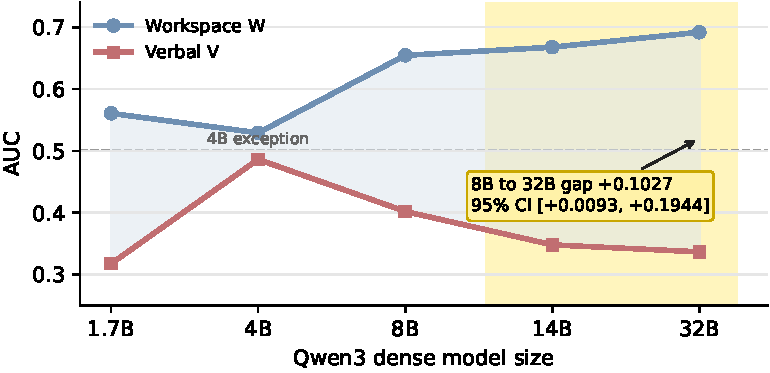
\includegraphics[width=0.82\textwidth]{figures/fig_v3_scale.pdf}
\caption{\updated{Corrected Qwen3 Decoupled scale sweep. Yellow shading marks
the newly added 14B/32B boundary region; the original figures elsewhere in
the paper are retained.}}
\label{fig:v3scale}
\end{figure}

\subsection{Limits of Static Readouts}
\label{sec:boundary}

The workspace readout does not recover every class of inferred content, and the
boundary is informative.
On Compositional, where the bridge is weakly evoked and matters only through a two-hop
composition, $\Wrr$ sits at chance for Qwen and OLMo (Mistral: $0.60$). This limitation is not an artifact of an untrained readout. Taking recovery
to mean a paired improvement over the static readout at 7B whose 95\% CI
excludes zero, a tuned future-token lens initialized at the model's own
unembedding and trained on disjoint contexts
\citep{pal2023futurelens,belrose2023tuned} does not recover Compositional
($+0.049$ $[-0.053, +0.149]$ at 7B; its only paired gain is at 0.5B, where
the absolute AUC remains near chance) and is significantly worse than the
plain logit lens on evoked bridges at 7B ($-0.088$;
App.~\ref{app:futurelens}). Across every static readout we tested, including a conditional-likelihood
score that is predictively comparable elsewhere (LL$-W$ on Compositional
$+0.078$ $[-0.040, +0.188]$, not a recovery under the paired criterion;
App.~\ref{app:vrobust}), the end-of-encoding state holds inferences that the
narrative actively evokes, rather than everything a future question might
make relevant. \S\ref{sec:extensions}
shows a gradient-based readout crosses this boundary in one of the two
families tested.

\textbf{Post-training analysis.}
In our stage sweep, none of 11 transitions improves the workspace channel:
eight Qwen base$\to$instruct pairs are flat to slightly negative, and OLMo-2's actual
pipeline declines cumulatively (base $0.631 \to$ SFT $0.599 \to$ DPO $0.576
\to$ RLVR $0.580$; $-0.052$, directional: one-sided $p{=}0.041$, two-sided
cluster CI $[-0.105, +0.007]$; App.~\ref{app:olmo}). What is unambiguous is
the absence of improvement in any of the 11 transitions. The
verbal channel's inferential-regime failure is not created by chat tuning:
raw-probed base models are erratic on inferred content (e.g., Qwen-7B
base $V_{raw}{=}0.11$ on Compositional; OLMo-2-1B base $0.445$), and the chat-tuned probe
settles at a confidently miscalibrated $0.27$--$0.30$. Post-training rewards are computed on emitted text, never on internal
availability, and the result is a fluent report channel that was never trained
against the internal one. (Scope: this concerns utility-salience; \citet{latentintrospection2026} show
that detection of injected concepts can be elicited in models, a different
construct, attributed there to in-context information rather than a
post-training mechanism.)

\begin{figure}[t]
\centering
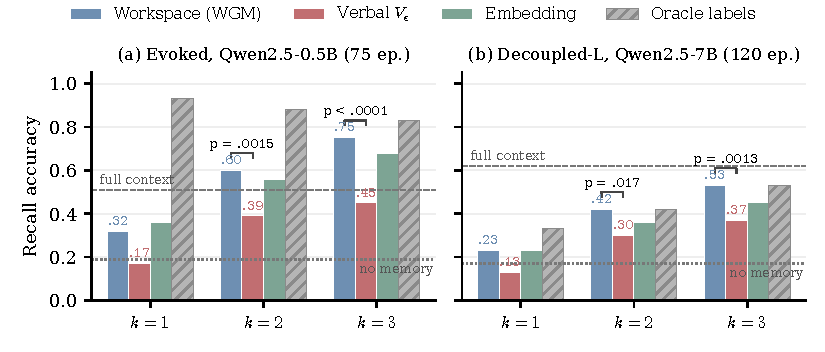
\includegraphics[width=\textwidth]{figures/fig3_downstream.pdf}
\caption{Budget-limited recall QA. Left: 0.5B on the Evoked benchmark, where
workspace gating beats verbal gating ($k{=}2$: $+20/-4$, $p{=}0.0015$; $k{=}3$: $+24/-2$,
$p{<}10^{-4}$), which sits at the no-memory floor. Right: 7B on the
construct-valid Decoupled benchmark (64-token answers), where workspace gating
matches the label oracle and beats verbal gating ($k{=}3$, $\dagger$: $+26/-7$, $p{=}0.0013$,
computed on the 120-episode scaled benchmark). The two panels are the two
regimes' primary cells; the full grid, which also contains null and reversed
cells at these $n$'s, and all McNemar tests are in
App.~\ref{app:downstream}.}
\label{fig:downstream}
\end{figure}

\subsection{Budget-Constrained Memory Selection}
\label{sec:payoff}

Fig.~\ref{fig:downstream} evaluates the two channels as write-admission policies.
At 0.5B on evoked bridges, gating on the binary importance probe stores
confidently wrong vivid words and at $k{=}1$ performs at the no-memory
floor, while workspace gating reaches $0.75$ at $k{=}3$; the paired advantage
is significant despite only 75 episodes. Budget-$k$ payoff tracks
within-episode ranking rather than the pooled AUC of Eq.~\ref{eq:auc}
(top-3 containment $0.707$ here; App.~\ref{app:downstream}). The canonical 1--10 rating variant is a
stronger verbal baseline on this answer-coupled benchmark (matching workspace
there) but sits at chance predictively on the construct-valid Decoupled benchmark
(App.~\ref{app:vrobust}).
At 7B on the $120$-episode construct-valid benchmark (Decoupled-L),
workspace gating shows no detectable
difference from the selection
oracle ($0.525$ vs.\ $0.525$ at $k{=}3$; paired difference $0.000$, 95\% CI
$[-0.092, +0.083]$; workspace nominally exceeds
the oracle in two other cells, indicating the oracle itself is noise-limited
at this $n$) and beats verbal gating on the same set
($+26/-7$, $p{=}0.0013$). Recency, random, and
the surface-feature fusion proxy lose to workspace gating throughout
(App.~\ref{app:downstream}, \ref{app:fusion}); embedding gating is the strongest
alternative but never separates from workspace downstream and is predictively
dispatched on Decoupled. Two boundary conditions: at 3B on Decoupled-class tasks the recall-time
composition step, not selection, is the binding constraint (oracle
$0.43$ vs.\ full-context $0.57$), and with a 24-token answer budget even the
oracle collapses: when the model cannot exploit a stored item at recall time,
selection quality has no effect.

\updatedparagraph{The workspace-only and oracle arms above are invariant to
the verbal-score migration. Direct comparisons that depend on the historical
Original verbal selected sets are treated as legacy evidence until their
selected sets are regenerated under v3; the new RL-QA comparison in
\S\ref{sec:newexperiments} uses a fully regenerated corrected Original arm.}

\begin{table}[t]
\centering
\caption{\textbf{Causal effect of input-side bridge steering on recall-time
answer preferences.} Real steering moves the residual stream from the
stored bridge toward a target bridge; sham uses an unrelated, norm-matched
direction. Qwen2.5 and Qwen3 checkpoints; 20 disjoint episode pairs.
A flip is a sign change in first-token target-versus-stored answer log-odds,
$\log P(a_{\rm target})-\log P(a_{\rm stored})$. Exact McNemar tests compare
paired real-versus-sham flips; exact two-sided Wilcoxon signed-rank tests
compare paired log-odds shifts. Specificity is strongest at gentle scales.}
\label{tab:causal}
\small
\begin{tabular}{llccccc}
\toprule
Model & Scale & Real flip & Sham flip & McNemar & $p$ & Wilcoxon $p$ \\
\midrule
Qwen2.5-7B & 0.5 & 0.70\dgain{+0.65} & 0.05 & $+13/-0$ & 0.0002 & 4.8e-05 \\
Qwen2.5-7B & 1.0 & 0.90\dgain{+0.60} & 0.30 & $+12/-0$ & 0.0005 & 1.9e-06 \\
Qwen2.5-3B & 0.5 & 0.60\dgain{+0.50} & 0.10 & $+11/-1$ & 0.0063 & 1.3e-04 \\
Qwen2.5-3B & 1.0 & 0.85\dgain{+0.50} & 0.35 & $+10/-0$ & 0.0020 & 3.8e-06 \\
Qwen2.5-0.5B & 1.0 & 0.75\dgain{+0.55} & 0.20 & $+11/-0$ & 0.0010 & 1.7e-04 \\
Qwen3-8B & 0.5 & 0.90\dgain{+0.75} & 0.15 & $+15/-0$ & 0.0001 & 1.9e-06 \\
Qwen3-8B & 1.0 & 0.95\dgain{+0.60} & 0.35 & $+12/-0$ & 0.0005 & 5.7e-06 \\
\bottomrule
\end{tabular}
\end{table}


\subsection{Causal Analysis}
\label{sec:causal}

The predictive results alone do not establish that the answer computation uses
the representations the readout measures; this section shows that it does.
To test this directly, we steer the residual stream along the stored bridge's
input-side difference-of-means direction \citep{zou2023repe} toward a
different bridge while the model answers from memory, versus sham directions
built from unrelated bridges on held-out episodes (20 disjoint pairs;
Fig.~\ref{fig:causal}).
Table~\ref{tab:causal}: at the gentlest scale the real direction flips the
answer in $0.60$ of pairs versus $0.10$ for sham at 3B (McNemar $+11/-1$,
$p{=}0.0063$) and in $0.70$ versus $0.05$ at 7B ($+13/-0$,
$p{=}2.4\times10^{-4}$), directionally consistent at 0.5B (tested at scale $1.0$). A flip means the
answer log-odds between the stored and the steered-toward bridge change
sign; sham directions are built from unrelated bridges of held-out episodes
at matched norm. At stronger steering scales real flips rise further but
sham flips rise too (App.~\ref{app:causal}), so the gentle-scale contrast
carries the specificity claim. Output-side (unembedding) steering has no effect, consistent with
\citet{anthropic2026workspace}. The concept representations the readout scores are therefore causally used
by memory-based answering; steering the unembedding rows (the output side)
does nothing, so the readout taps content, not output preparation.

\subsection{Gating Evaluation}
\label{sec:prgresults}

\begin{table}[t]
\centering
\caption{Write-admission policies on the mixed-provenance pool
(Explicit $\cup$ Evoked $\cup$ Decoupled-L; 283 episodes; per-benchmark
generation budgets fixed across policies; all cells from a single run
generation). Bold: column best among content-scoring policies; the two internal signals
(likelihood, workspace) are statistically indistinguishable in every cell
(all $p{\ge}0.10$) and each beats the binary probe. The absence heuristic
exploits the single-planted-inference construction and collapses on
multi-absent pools (three-act analysis, App.~\ref{app:prg}); pairwise tests
and the 1--10 rating analysis are also there.}
\label{tab:prg}
\small
\begin{tabular}{lcccc}
\toprule
\multirow{2}{*}{Policy} & \multicolumn{2}{c}{0.5B} & \multicolumn{2}{c}{7B} \\
\cmidrule(lr){2-3} \cmidrule(lr){4-5}
 & $k{=}2$ & $k{=}3$ & $k{=}2$ & $k{=}3$ \\
\midrule
Verbal (binary probe) & 0.290 & 0.329 & 0.463 & 0.555 \\
Verbal (1--10 rating) & 0.343 & 0.410 & 0.491 & 0.601 \\
Embedding & 0.350 & 0.442 & 0.477 & 0.583 \\
Cond.\ likelihood (one pass/cand.) & \textbf{0.375} & \textbf{0.466} & \textbf{0.537} & 0.618 \\
\wsrow Workspace (zero passes) & 0.332 & 0.431 & 0.502 & \textbf{0.636} \\
PRG (routed) & 0.336 & 0.417 & \textbf{0.512} & 0.565 \\
\addlinespace
\refrow Absence heuristic (diagnostic) & 0.459 & 0.459 & 0.629 & 0.636 \\
\refrow Oracle & 0.512 & 0.484 & 0.657 & 0.707 \\
\bottomrule
\end{tabular}
\end{table}

Table~\ref{tab:prg} evaluates the gate in the deployment-realistic setting: a
pooled stream mixing all three provenance regimes, where any channel that
fails on one regime pays for it. Because the contribution is an admission
score rather than a memory system, the comparison holds the pipeline fixed
and varies only the score; an end-to-end comparison against full memory
frameworks would confound retrieval, organization, and prompting with the
admission signal under study, and every such framework can adopt whichever
score wins here. Three results follow.

\myparagraph{The workspace gate beats the binary probe.}
Replacing the
binary importance probe with the workspace readout wins at $k{=}3$ at both
scales ($+47/-18$, $p{=}0.0004$, confirmatory under Holm correction over the
full test family; $+45/-22$, $p{=}0.0067$ uncorrected, marginal after
correction; App.~\ref{app:prg}),
and the workspace channel is never significantly worse than any
content-scoring policy in any cell.

\myparagraph{The failure is specific to the verbal channel, not to internal signals generally.}
Against the canonical 1--10
rating, the strongest verbal form, workspace gating is numerically ahead at
7B ($0.636$ vs.\ $0.601$, $p{=}0.31$) at zero probe cost, where the rating
spends one forward pass per candidate, and on the construct-valid slice the
rating is predictively at or below chance (App.~\ref{app:vrobust}). An
internal conditional-likelihood score at that same one-pass cost gates
indistinguishably from the workspace readout (all cells $p{\ge}0.10$) and
itself beats the binary probe ($p{\le}0.035$ in three of four cells,
$p{=}0.051$ in the fourth; App.~\ref{app:prg}); the readout is the internal
signal that needs no extra passes and carries the causal grounding of
\S\ref{sec:causal}.

\myparagraph{At tight budgets, provenance routing adds a little more.}
At the tight 7B budget provenance routing is the strongest policy
that spends no per-candidate forward passes ($0.512$ vs.\ $0.502$
single-channel) and helps where the channels are complementary; the single-channel
gate is the recommended default at capable scale. Calibration matters:
$z$-normalized routing loses admission slots for inferred items
systematically because the two score distributions differ in shape, and
underperforms rank calibration throughout (App.~\ref{app:prg}). Finally,
because each benchmark plants a single inference, bare absence is nearly an
oracle proxy here; App.~\ref{app:prg} analyzes this diagnostic and the
multi-absent stress tests, where the degenerate absence heuristic collapses
and, when the competing absent candidates are semantically confusable, the
workspace readout is the leading channel: its selection-signal advantage
over the embedding replicates on a fresh 120-episode set (paired
$\Delta$AUC $+0.064$, one-sided $p{=}0.026$; pooled estimate $+0.058$
$[+0.007, +0.108]$) and gated QA shows no
detectable difference from the true-label oracle (App.~\ref{app:prg}).
On the two standard naturalistic streams (LoCoMo, LongMemEval), whose
candidates are surface content by construction, no question-blind channel,
ours or the verbal importance probe, separates from random under LLM-judge
grading:
the construct that separates the channels is structurally absent there, which
is precisely why the controlled benchmarks of \S\ref{sec:benchmarks} are
needed. When that construct is planted back, by embedding our Decoupled
episodes inside real LoCoMo sessions, the dissociation reappears at 7B with
the workspace readout unattenuated ($W{-}V$ $+0.21$ $[+0.10, +0.31]$): the
effect is carried by content provenance, not by synthetic style
(App.~\ref{app:locomo}).
